% Chapter 2

\chapter{导航卫星精密轨道确定的基础原理}

\section{引言}

正如前述所说,提供实时高精度的导航卫星轨道服务对当前实时高精度定位具有重要意义,而导航卫星精密轨道确定的核心任务,就是利用长时间连续弧段的高精度GNSS观测信息,确定导航卫星在该时间弧段内的空间位置信息。
因此轨道确定中的其中一个常用的方法即为几何学定轨法(Bisnath et al. 1999;韩保民,2003) ,其核心原理与定位过程类似,利用高精度GNSS观测值直接交汇计算出目标体的动态位置。这类方法常常用于低轨卫星的轨道确定中,而对导航卫星,受限于地面观测几何构型,使用效果不足以满足当前对轨道精度的需求。

除利用高精度GNSS观测信息外,导航卫星自身的运动规律信息同样可以应用于定轨中。
考虑到导航卫星在空间环境中主要受到地球的万有引力作用,因而其具有围绕地球的类椭圆的周期性的运动轨迹。若将卫星和地球均视为质点,此时导航卫星的运动可被简化为一个二体问题。根据天体力学原理,其运动轨迹可被六个轨道参数所确定,此时轨道确定问题转化为轨道参数的确定。然而在导航卫星实际的运动过程中,除主要的地球万有引力,还会受到到其他摄动力的影响(如地球非球形引力、地球潮汐引起的引力摄动、地球辐射等等),此时将难以构建类似二体问题中轨道参数的解析表达式描述卫星的运动轨迹。在这种情况下,假定受力模型已知,导航卫星的运动轨迹信息可以通过数值积分的得到。动力学定轨法(刘林,1992)正是结合了导航卫星的运动模型和GNSS几何观测信息进行轨道确定,其通过动力学方程来维系导航卫星连续弧段内的位置信息,其显著改善了仅使用GNSS观测信息定位所带来的误差,因此导航卫星动力学模型的构建是动力学定轨法中的一个关键部分。

接下来本章就针对对导航卫星动力学定轨法中所涉及的基础算法原理进行梳理和介绍。首先是有关导航卫星位置信息表述中常用的时空参考系统,然后就动力定轨法所涉及的GNSS观测模型以及导航卫星的运动模型进行基本阐述。

\section{时空参考系统}

\subsection{时间系统}

时间系统的参考基准是由起始历元和时间尺度两者所确定的。目前常用的时间系统根据其定义和用途,主要可以分为以下三种类别:
\begin{enumerate}
    \item 以地球自转规律为基础所定义的世界时系统。常见的包括恒星时(Sidereal Time,ST),以及世界时(Universal Time,UT)。
    \item 以天体运动方程为基础所定义的力学时系统。常见的包括地球时(Terrestrial Time,TT)和太阳质心动力学时(Barycentric Dynamical Time,TDB)。
    \item 以原子运动规律为基础所定义的原子时系统。常见的包括国际原子时(temps atomique International,TAI),协调世界时(Barycentric Dynamical Time,UTC)
\end{enumerate}

尽管目前四大全球卫星导航系统定义了各自的时间系统作为参考基准,但它们都是属于原子时一类的时间系统。即它们的时间尺度相同,只是在定义起始历元上有所区别。图~\ref{fig:timerefer}给出了常见的时间系统之间的转换关系 。
\begin{figure}
  \centering
  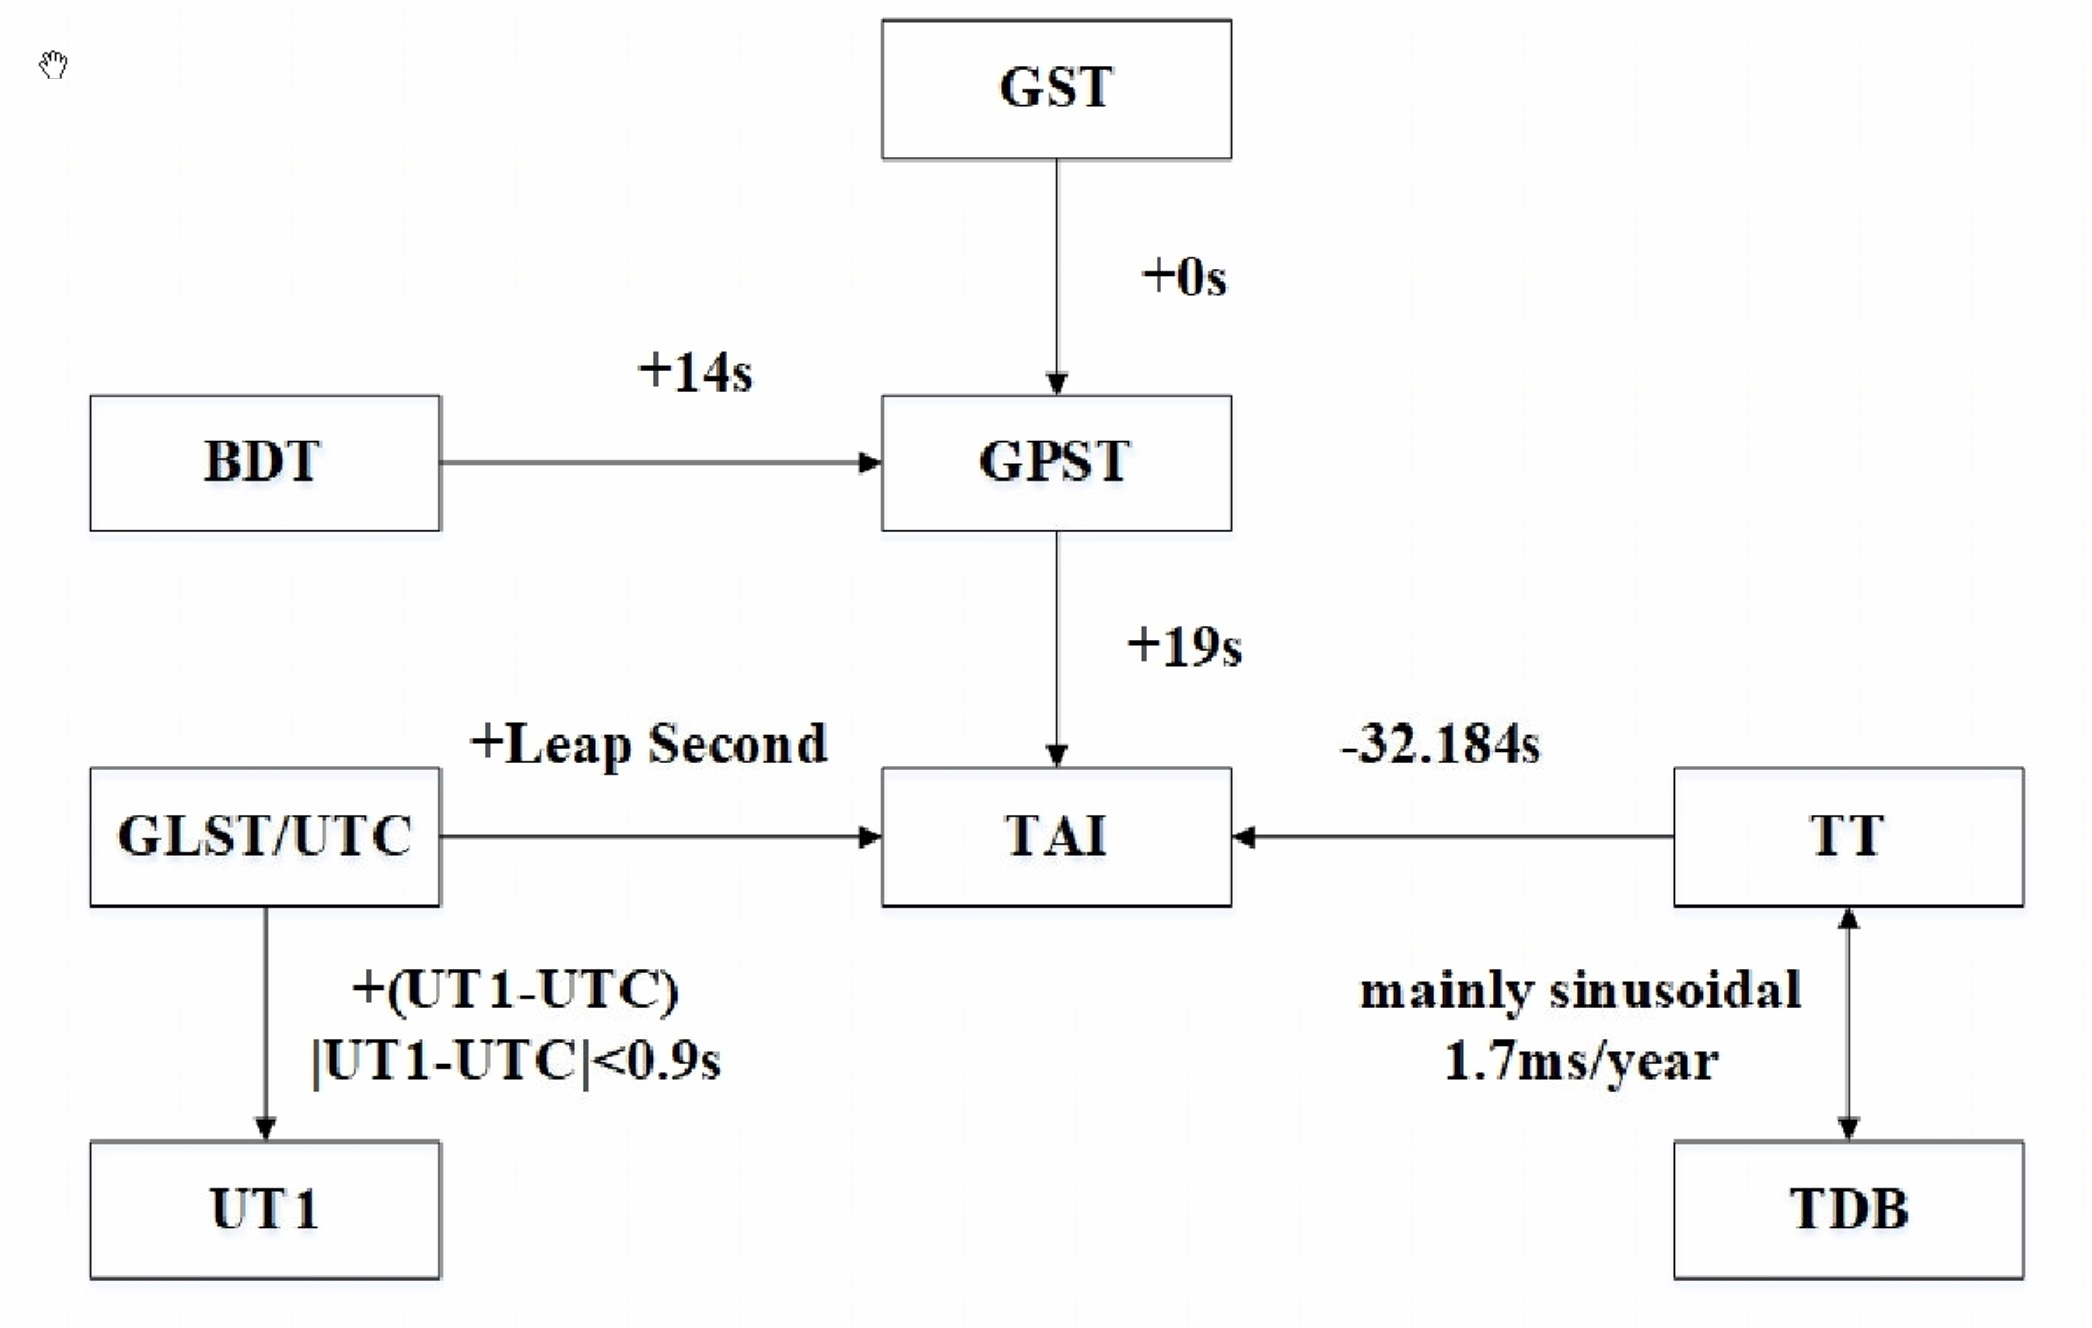
\includegraphics[width=1\textwidth]{timerefer.png}
  \caption{各常见时间系统转换示意图}
  \label{fig:timerefer}
\end{figure}

\subsection{坐标系统}

坐标系统的参考基准是由坐标原点、坐标轴指向以及坐标轴尺度这三个方面所确定的。在导航卫星精密轨道确定过程中,常常涉及多个不同坐标系所描述的位置信息,通常需要归算至同一坐标参考系统中。因此明确各个坐标系统的定义以及它们之间的转化关系尤为重要。下面对定轨过程中涉及的常见坐标系统做一个介绍。
\begin{itemize}
    \item 地心固体坐标系统

    地心固体坐标系统通常指的是一类具有跟随地球自转、与地球固连特性的坐标系统。由于该坐标系统的定义更为符合人们日常生活的直观感受,因此常常应用于许多科学应用活动中,如固定测站的坐标描述、地球重力场模型、地球潮汐模型等。
    由于地球本身极移等特性,很难在实际空间中找到地心固体坐标系统的参考标志,因此地心固体坐标系的定义是一种人为协议的结果。其中由国际地球自转服务(International Earth Rotation Service,IERS)所提出的国际地球参考系(International Terrestrial Reference System,ITRS)是目前国际上所公认采用的一种标准。几乎所有的地心固体坐标系的定义与ITRS保持或接近一致。
    而对于地心固体系统具体实现,则是通过维持一组参考点的位置和和速度完成。IERS就通过多种空间大地测量技术以及相应的全球参考站维护了一套国际地球参考框架(International Terrestrial Reference Frame,ITRF),也是目前最为完善、精度最高的地心固体坐标系的实现。除此之外,对各个导航卫星系统而言,由于其构建和使用的地心固体坐标系在定义或是实现坐标系的参考站上的不一致,也衍生出了不同的地心固体坐标系。GPS系统的广播星历即是以WGS84坐标系(World Geodetic System)为基础,类似的GLONASS系统使用的为PZ90坐标系以及Galileo使用的为GTRF坐标系。对于我国的北斗导航卫星系统而言,一开始使用的为2000中国大地坐标系(China Geodetic Coordinate System 2000,CGCS2000),而后从2017年12月开始,开始使用北斗坐标系统(BeiDou Coordinate System,BDCS)(魏子卿等, 2019)。 

    \item 惯性坐标系统

    前述的地心固体坐标系统由于会随地球自转不断发生改变,因此难以在该坐标系统下构建导航卫星的动力学方程,而惯性坐标系统则更适用于导航卫星运动描述。
    在天文学中,天球参考系通常用来作为描述天体运动的惯性坐标系统。类似地,以地球质心为原点的地心赤道天球坐标系统常被用于导航卫星运动的描述中。在该坐标系统中,天极(即地理极点在天球上的投影)以及赤道面上的春分点被用于标定坐标轴的指向。
    但由于地球岁差和章动的影响,赤道天球坐标系统同样是随时间缓慢变化的,这对后续科学活动中的使用依然十分不方便。因此国际天文联合会(International Astronomical Union,IAU)提出了J2000.0的协议天球坐标系,其即对应的着TDB为2000年1月1日12时的赤道天球坐标系统。
    在导航卫星轨道确定中,由于地球参考站常常使用地心固体坐标系,因此常常涉及其与天球坐标系之间的转换,从前述两者的定义可知,通过对地球岁差、章动、极移、自转进行相应的分析,即可获得两者坐标系之间的旋转矩阵(李征航等,2010)。
    \item 卫星轨道坐标系统
    
    由于对卫星轨道精度以及力学模型进行评价时候,常常需要分析其在卫星瞬时速度方向及与地球质心连线方向上的分量大小,因此引入了对应的卫星轨道坐标系。该坐标系的三个方向分别由径向(Radial)、切向(Along-track)和法向(Cross-track)所构成,其具体定义可参照如下公式\eqref{eq:ACR_ref}:
    \begin{equation}
        \begin{aligned}
        \vec{R} & =\frac{\vec{r}}{|\vec{r}|} \\
        \vec{C} & =\frac{\vec{r}\times\vec{v}}{|\vec{r}\times\vec{v}|} \\
        \vec{A} & =\vec{C}\times\vec{R} \\
        \end{aligned}
        \label{eq:ACR_ref}
    \end{equation}
    式中,\(\vec{r}\)表示导航卫星的位置向量,\(\vec{v}\)表示导航卫星的速度向量,\(\vec{R},\vec{C},\vec{A}\)分别表示坐标系的径向、法向和切向。

    \item 星固系

    为了方便描述导航卫星上的如天线相位中心偏差、卫星天线相位缠绕等相关问题,因此引入星固坐标系。由于不同导航卫星天线制造与控制上的差异,具体星固系的定义也有所区别。这里以IGS定义的协议星固系为例:该坐标系统的原点定义在卫星质心,其中以太阳帆板旋转轴为Y轴,同时理论上天线所指地心方向为Z轴,最终X轴可由Y轴和Z轴所构成的右手坐标系唯一确定(Montenbruck 等, 2015)。


\end{itemize}

\section{GNSS观测模型}

这里参考下当时写IFCB论文里面的观测模型吧,相应的误差改正就简单的概况一下吧。

\section{导航卫星运动模型}

\subsection{动力学方程和状态转移}

\subsection{摄动力模型}

\section{参数估计方法}
目前高精度 GNSS 数据处理的方法主要可以分为两大类,一类是最小二乘估计,一类是卡尔曼滤波估计。卡尔曼滤波通过递推的方式,利用参数的协方差信息 阵(实际上是包含了参数的先验信息以及之前所有历元的观测信息)以及当前历元 的新增观测数据,通过时间更新、状态更新两个步骤,给出了基于最小方差准则下 的参数最优估计值以及相应的协方差[21]。而最小二乘,则是根据相应观测量组建 观测方程,考虑观测量的随机模型,给出了基于最小残差平方和下的参数最优估计 值。虽然二者表现形式不同,其本质上是一样的
\subsection{最小二乘}

参考下本科设计时候的思路写一下这部分的内容

\subsection{卡尔曼滤波}

参考之前整理的推导的卡尔曼滤波内容的部分下一下这部分的内容
